% Choose the report format
\documentclass[11pt]{article}
\usepackage[
    a4paper,
    left=20mm,
    right=20mm,
    top=20mm,
    bottom=20mm
    ]{geometry}
\renewcommand{\baselinestretch}{2}
\usepackage{setspace} % set 1.5 spacing
\onehalfspacing
\usepackage{helvet} % set font type
\renewcommand{\familydefault}{\sfdefault}
\usepackage{fancyhdr}

% Encoding parameters (always necessary ?)
\usepackage[utf8]{inputenc}
\usepackage[T1]{fontenc}
\usepackage[french]{babel}

% Make some reference, bibliography and others
\usepackage{biblatex}
\addbibresource{biblio.bib}

\usepackage{wrapfig}
\usepackage{hyperref}
\usepackage{caption}

% For the math symbol in latex equations
\usepackage{amsmath}

% For 
\usepackage{graphicx}
\graphicspath{{../fig/} }

\begin{document}
    
    %-------------------------
    % Page de Garde
    %-------------------------

    \pagestyle{fancy}
    \fancyfoot{}
    \fancyfoot[L]{Aix-Marseille Université}
    \fancyfoot[R]{2023/2024}
    \vspace{5cm}

    \begin{center}
        \Large \textbf{Analyse du report des voix entre les deux tours des élections législatives anticipées de 2024.}
    \end{center}
    
    \vspace{2cm}
    
    \begin{center}
        Mémoire en vu de l'obtention du Diplôme d'Etudes Supérieures Universitaires de Data Science \\
        \textit{par Alexandre Lainé}
    \end{center}

    \newpage
    % Document format
    \pagestyle{fancy}
    \fancyhead{} % clear all header fields
    \fancyhead[L]{Alexandre Lainé}
    \fancyhead[R]{Mémoire DESU de Data Science}
    \fancyfoot{} % clear all footer fields
    \fancyfoot[R]{\thepage}

    %-------------------------
    % Intro, Question Scientifique et Contexte (1page)
    %-------------------------
    \section{Introduction}

    Peu après les élections européenne 2024 auxquelles la liste du Rassemblement National (RN), porté par Jordan Bardella et Marine Le Pen, a obtenu 37 \% des suffrages \cite{Le_Monde_2024a}. Le Président de la République a décidé de dissoudre l'Assemblée Nationale et ainsi déclencher des élections législatives anticipées. Après un premier tour record pour le RN, c'est finallement le Nouveau Front Populaire (NFP ou Union de la Gauche, UG) qui est arrivé en tête (182 sièges) après un entre deux tours rythmé par les désistements et les consignes de votes afin de faire barrage au RN dans un maximum de circonscriptions \cite{Wikipédia_2024a}. 

    \begin{wrapfigure}{R}{0.4\textwidth}
        \begin{center}
            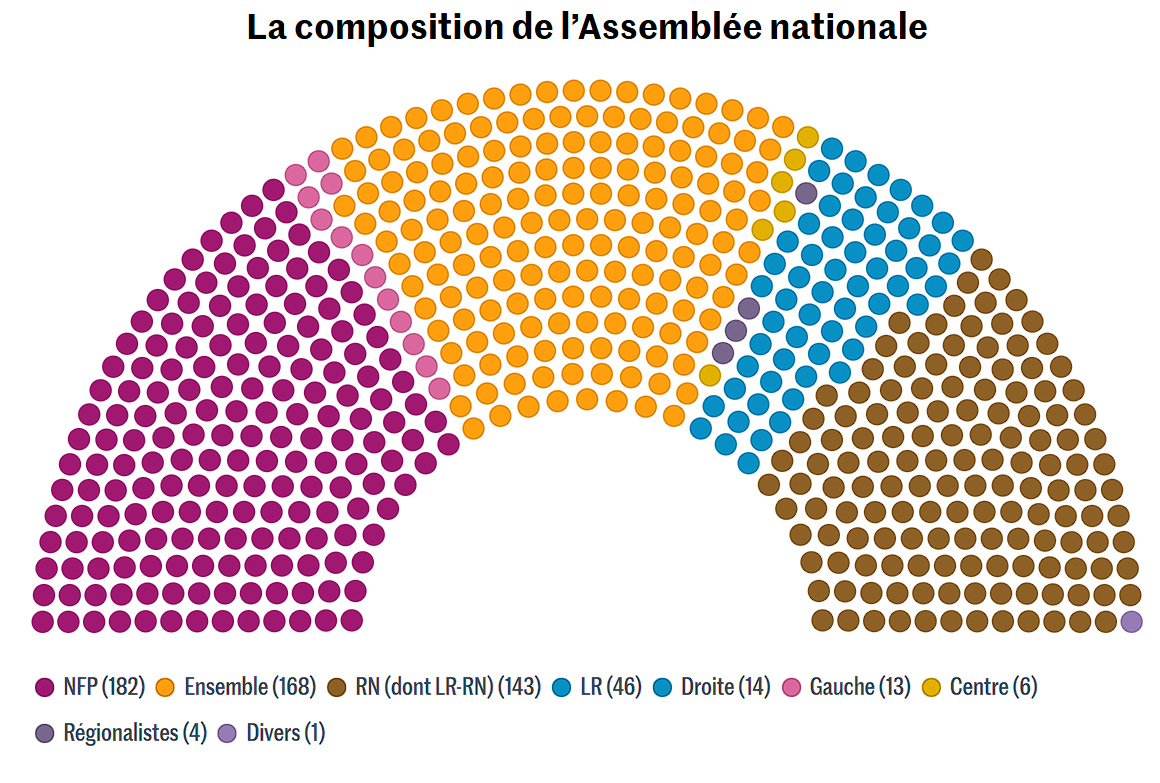
\includegraphics[width=0.38\textwidth]{Resultats_2024.png}    
        \end{center}
        \caption{Répartition de l'assemblée nationale suite aux élections législatives anticipées de 2024 \cite{Le_Monde_2024b}.}
    \end{wrapfigure}

    Ces mouvements de voix sont particulièrement interressant, et il est possible de se demander si les résultats du premiers tour sont suffisant pour prédire le dérouler du second. Basée sur cette interrogation, il s'agirait par conséquent de trouver une règle décrivant les mouvements de voix entre les deux tours. Depuis la publication des résultats, très peu de travaux ont été publié. La seule approche utilisé à ma connaissance, et ne se basant sur des sondages, est celle de l'apprentissage statistique \cite{Amblard_2024} visant à estimer le taux de report entre les familles politiques. Celui-ci prend alors la forme d'une distribution sur l'ensemble des circonscriptions décrite par une moyenne et une variance particulière. Néanmoins cette approche ne répond pas tout à fait à la question posée, en guise de base à ce travail, il a déjà été décrit une approche d'apprentissage automatique permettant d'estimer le transfert des voix entre les deux tours des élections présidentielles de 2022 sous la forme d'une matrice \cite{Perrinet_2022}. Néanmoins, dans notre cas des élections législatives, le problème est plus complexe, car dans chaque circonscription les nuances des candidats du second tour peuvent être différentes. Cela ajoute par conséquent à l'hétérogénéïté des bureaux de vote une forte diversité quand au grand nombre de faces à faces possibles. 

    L'objectif de ce projet est donc d'utiliser cette approche d'apprentissage automatique afin de trouver une matrice représentant le taux de transfert de voix de chaque partie du premier tour vers ceux du second tour. Il est alors nécessaire de passer par plusieurs niveau de complexité, tout d'abord en regroupant les différentes nuances politiques sous la forme de famille, puis de resteindre l'apprentissage qu'à des cas particulier de face à face, avant de tenter la phase la plus complexe en tentant l'apprentissage sur l'ensemble des bureaux de votes. Cependant, il est import de notifier quelques précisions. Tout d'abord, il est normalement impossible de trouver le taux réel de report entre deux nuances, car celui-ci est surement dépendant de paramètres géographiques et socio-économiques. Ensuite, ce taux de report généralise une règle pour l'ensemble d'un partie et passe donc au dessus des possibles divergences présentent. Enfin, s'agissant d'un sujet actuel, l'objectif n'est ici en aucun cas de "refaire le match" mais seulement d'utiliser des outils issues de l'intelligence artifielle afin d'analyser les données de ces élections en ce concentrant sur les mouvements de voix notamment dû à la mise en place d'un "front républicain". Ce terme, apparût pour la première fois à l'occasion des élections législatives de 1956, prend racine dans la défense républicaine qui a eu lieu au début de la troisième république afin de faire barrage aux élans monarchistes.
    
    \newpage
    %-------------------------
    % Matériel et Méthodes (3pages)
    %-------------------------
    \section{Matériel et Méthodes}

        \subsection*{Jeux de donnés}
            Résultats des élections législatives pour le premier et second tour pour chaque bureau de vote en France métropolitaine, dans les Territoires d'Outre Mer, mais aussi à  l'étranger. Il s'agit respectivement de fichier d'environ 40 et 16 Mo, renseignant pour chaque bureau de vote le nombre de voix obtenu par chaque candidat, ainsi que le nombre d'inscrit, le nombre d'abstension et le nombre de bulletin nul.
        
        \subsection*{Pré-processing des données}
            De façon général l'objectif de cette phase de préprocessing est de supprimer les colonnes ainsi que les lignes vides, mais aussi les informations qui ne nous seront pas nécessaire pour la suite : genre, nom et prénom du candidat, nom de la commune et du département, ainsi que les bureaux de votes n'ayant pas eu besoin de second tour car ceux-là ne peuvent pas nous renseigner sur le report de voix. Il est important de noter qu'avant toutes étape d'apprentisage, le jeu de donné est coupé en deux parties, la première permettant l'entrainement, et la seconde permettant d'évaluer la précision du modèle sans que cela soit pris en compte pour l'apprentisage. De plus, bien que le tableau ne soit composé que du nombre de voix obtenue par chaque nuance, la première étape dans la fonction d'apprentissage consiste à diviser le nombre de vote obtenue par chaque nuance au sein d'un bureau de vote par le nombre total de votes exprimés obtenue dans ce bureau de vote.

            Afin d'avoir une progression dans la complexité de la tâche d'apprentissage automatique, on différenciera trois façon de préparer le jeu de donné :
            \begin{itemize}
                \item[--] En regroupant les nuances en familles politiques. L'objectif a été ici de rassembler dans chaque bureau de vote les résultats des nuances présentents sous la forme de grand groupes, en se basant sur leur localisation dans l'éventail politiques \cite{Wikipédia_2024b}.
                \item[--] En se focalisant uniquement sur les bureaux de votes présentant des face-à-faces particuliers. Notament en se focalisant principalement sur sur ceux ayant généré beaucoup de report dû à la présence du Rassemblement National au second tour.
                \item[--] En conservant toute la complexité des élections, mais en supprimant tout de même le nombre d'abstention, de vote nul, ou de vote blanc.
            \end{itemize}

            Pour le regroupement sous la forme de "familles" a été réalisé comme suit :
            \begin{itemize}
                \item[--] EXTGAUCHE+ : Extrême gauche, France insoumise, Parti communiste, Parti radical de gauche.
                \item[--] GAUCHE+ : Union de la Gauche, Ecologiste, Socialiste, Divers gauche.
                \item[--] CENTRE+ : Ensemble, Horizon, Union des Démocrates et Indépendants, Divers centre.
                \item[--] DROITE+ : Les républicains, Divers droite.
                \item[--] Divers+ : Divers, Les écologistes, Droite souverainiste, Régionaliste.
            \end{itemize}

        \subsection*{Modèle de transfert de voix}
            Si on considère le pourcentage de voix obtenu par chaque partie dans un bureau de vote comme une distribution discrète notée $D$, l'hypothèse est qu'il existerait une matrice de transition $M$ permettant de faire le lien entre les distributions du premier et second tour (respectivement $D_1$ et $D_2$). Mathématiquement, cela s'exprimerait comme suit :
            \begin{equation}
                \hat{D_2} = D_1 \times M
            \end{equation}
            L'objectif est donc d'utiliser les résultats du premier et du second tour afin d'apprendre de façon automatique cette matrice $M$ de ($n$ lignes et $m$ colonnes correspondant respectivement au nombre de nuances au premier et au second tour). Ce modèle de transfert de voix sera donc constituer d'une couche d'entrée dont la taille correspond au nombre de nuances politiques présentent au premier tour dans toute la France, mais aussi d'une couche de sortie, dont la taille correspond au nombre de nuances présentent au second tour. La matrice $M$ correspond par conséquent aux poids reliant la première à la seconde couche. 


        \subsubsection*{Divergence de Kullback-Leilbler}
            La divergence de Kullback-Leilbler \cite{Kullback_Leibler_1951} ($KL$) est une mesure permettant la comparaison entre deux distributions de probabilités discrètres. Celle-ci nous permettra de comparer la distance entre les distributions réelles du second tour ($D_2$) et celles prédites par notre modèle ($\hat{D_2}$) selon la formule suivante :
            \begin{equation}
                KL(D_2,\hat{D_2}) = \sum_{k \in \Omega} D_2 \cdot \log \frac{D_2}{\hat{D_2}}
            \end{equation}

        \subsubsection*{Entrainement et contrôle}
            Bien qu'il soit possible d'incorporer une fonction de stop anticipé de l'apprentissage, le choix fait ici a été de tenter différents nombre d'itération et de stopper l'apprentisage dès que le résultats de la fonction de coût, pour la partie de validation, se stabilise. La descente de gradient est réalisée par une implémentation pytorch de l'agorithme d'optimisation Adam très efficace dans le cas d'un jeu de donné large et d'une optimisation d'un grand nombre de paramètres \cite{Kingma_Ba_2017}.

        \subsection*{Visualisation et représentations graphiques}
            Afin de visualiser le jeu de donné et de rendre compte des différents résultats obtenues dans cette pipeline, il a été choisis d'utiliser principalement les bibliothèques matplotlib (version 3.9.0) et seaborn (version 0.13.2) pour leurs simplicités d'utilisation mais aussi de découvrir plotly (version 5.24.0) pour la qualité de ses graphiques interactifs et sa capacité à gérer une grande quantité de données. La plus part des figures créer das la pipeline sont enregistrées de façon automatique en format pdf au sein du dossier "fig" de la pipeline.
            
        \subsection*{Information supplémentaires}
            L'ensemble des codes de la pipeline sont disponible en libre accès sur la plateforme GitHub en cliquant juste \href{https://github.com/alexandre-laine/Pipeline_Elections_Legislatives}{ici}. L'ensemble de l'analyse a été développée et écrite pour le mémoire du DESU avec le langage de programmation Python (version 3.11.9) majoritairement sous la forme de notebook appellant des fonctions écrite par mes soins. Les calculs ont été réalisé en local sur mon ordinateur personnel (OMEN by HP Laptop 16-xf0xx) ayant les caratéristiques ci-contre (CPU : AMD Ryzen 9 7940HS, GPU-1 : AMD Radeon 780M, GPU-2 : NVIDIA GeForce RTX 4070).

    \newpage
    %-------------------------
    % Résultats (4pages)
    %-------------------------
    \section{Résultats}
        
        \subsection*{Grandes familles politiques}
            
            Cette première partie vise à répondre d'une manière très simplifiée à la question en ne considérant que des grandes "familles" politiques. Il a été possible d'estimer la matrice de transition entre les deux tours comme on peut le voir sur la partie gauche de la figure \ref{fig:Famille} sur laquelle on remarque qu'un groupe au premier tour influence majoritairement son propre groupe au second tour. Sur la partie centrale de la figure \ref{fig:Famille}, on représente cette fois-ci les pourcentages prédit obtenue dans chaque bureau de vote en fonction des pourcentages réels afin d'avoir une idée du niveau de précision de la prédiction. Bien qu'une partie des points se situent bien sur la diagonale rouge, il est possible de distinguer deux groupes qui diffèrent de cette diagonale, soit par une sur-évaluation du nombre de voix, soit par une sous-évaluation de celui-ci.
            
            \begin{figure}[h]
                \begin{center}
                    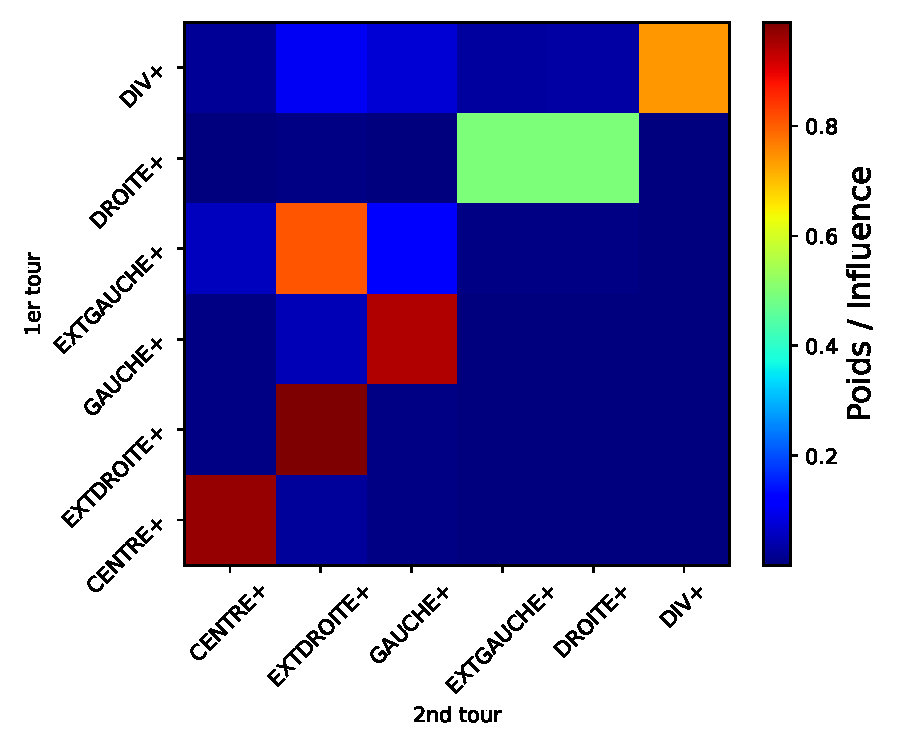
\includegraphics[width=0.25\textwidth]{Famille_Matrice.pdf}
                    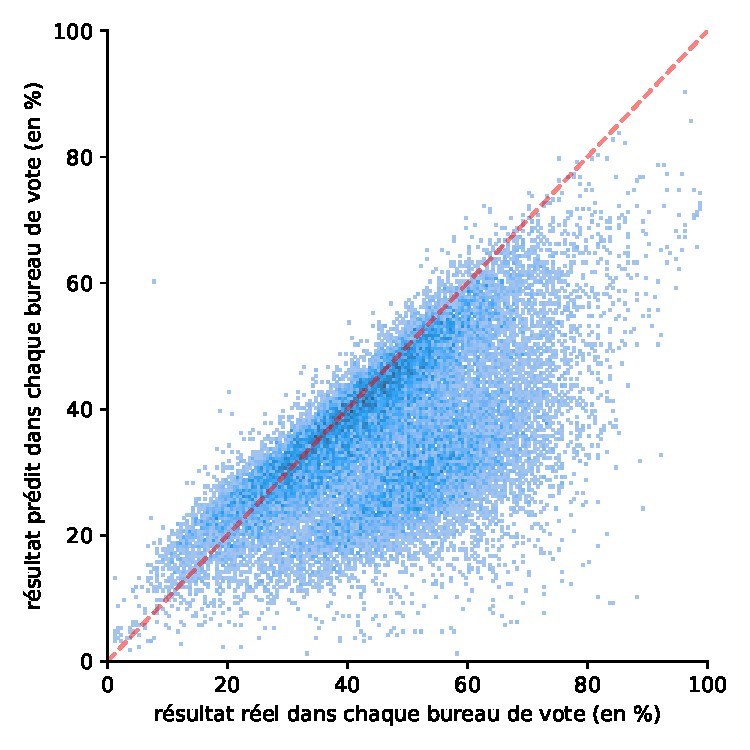
\includegraphics[width=0.25\textwidth]{Famille_True_Pred_Hist.pdf}
                    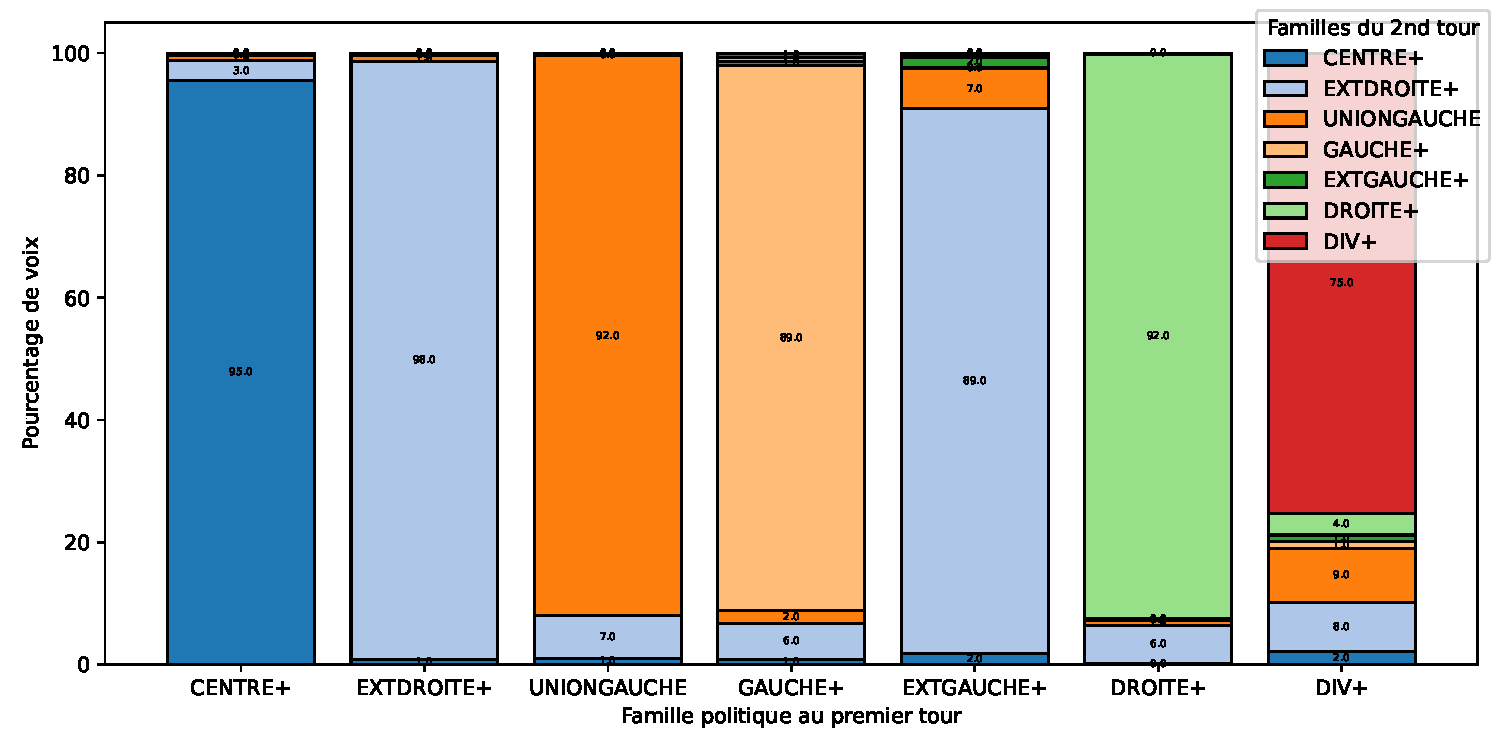
\includegraphics[width=0.4\textwidth]{Famille_Proportions.pdf}
                    \caption{Gauche) Matrice de transition de l'entre deux tour estimée. Centre) Comparaison entre les valeurs prédites et réelle par le biai un d'un histogramme en deux dimensions. Droite) Représentation estimée de chaque familles du premier tour dans les résultats des familles du second tour.}
                    \label{fig:Famille}
                \end{center}
            \end{figure}

        \subsection*{Face-à-face}

            Afin de complexifié la tâche, il est possible de se focaliser uniquement sur les bureaux de vote présentant des face-à-face pour étudier le report des voies de façon plus spécifiques. Le premier élément nous confirmant que l'apprentissage de la matrice de transition s'est bien déroulé, est résumé au niveau de la figure \ref{fig:Focus_pred_true}. On remarque qu'à l'inverse de la précédente figure, on ne remarque cette fois-ci aucun autre groupe que celui présent sur la diagonale.

            Cette seconde partie aurait donc mieux fonctionné. Comme vérification post-analyse, il est possible de représenter le pourcentage de report de chaque partie du premier tour en fonction de la nuance du candidat présent au second tour. On remarque alors rapidement des mouvements pouvant sembler logique, avec un report des voix de l'Union de la Gauche évitant toujours le Rassemblement National (figures \ref{fig:ENS-RN} et \ref{fig:LR-RN}), avec 90\% et 85\% de report respectivement vers Ensemble et les Républicain. De la même façon, mais en de moindre mesures Ensemble présente un report de 70\% vers l'Union de la Gauche, et de 80\% vers les Républicains (figures \ref{fig:LR-RN} et \ref{fig:UG-RN}). Pour ce qui est des nuances rares, les pourcentages de report sont plutôt équivalent, surement à cause du faible nombre d'exemple, sauf dans le cas de fortes affinitées politiques (DVG et EXG vers UG, REC vers RN).

            \begin{figure}
                \begin{center}
                    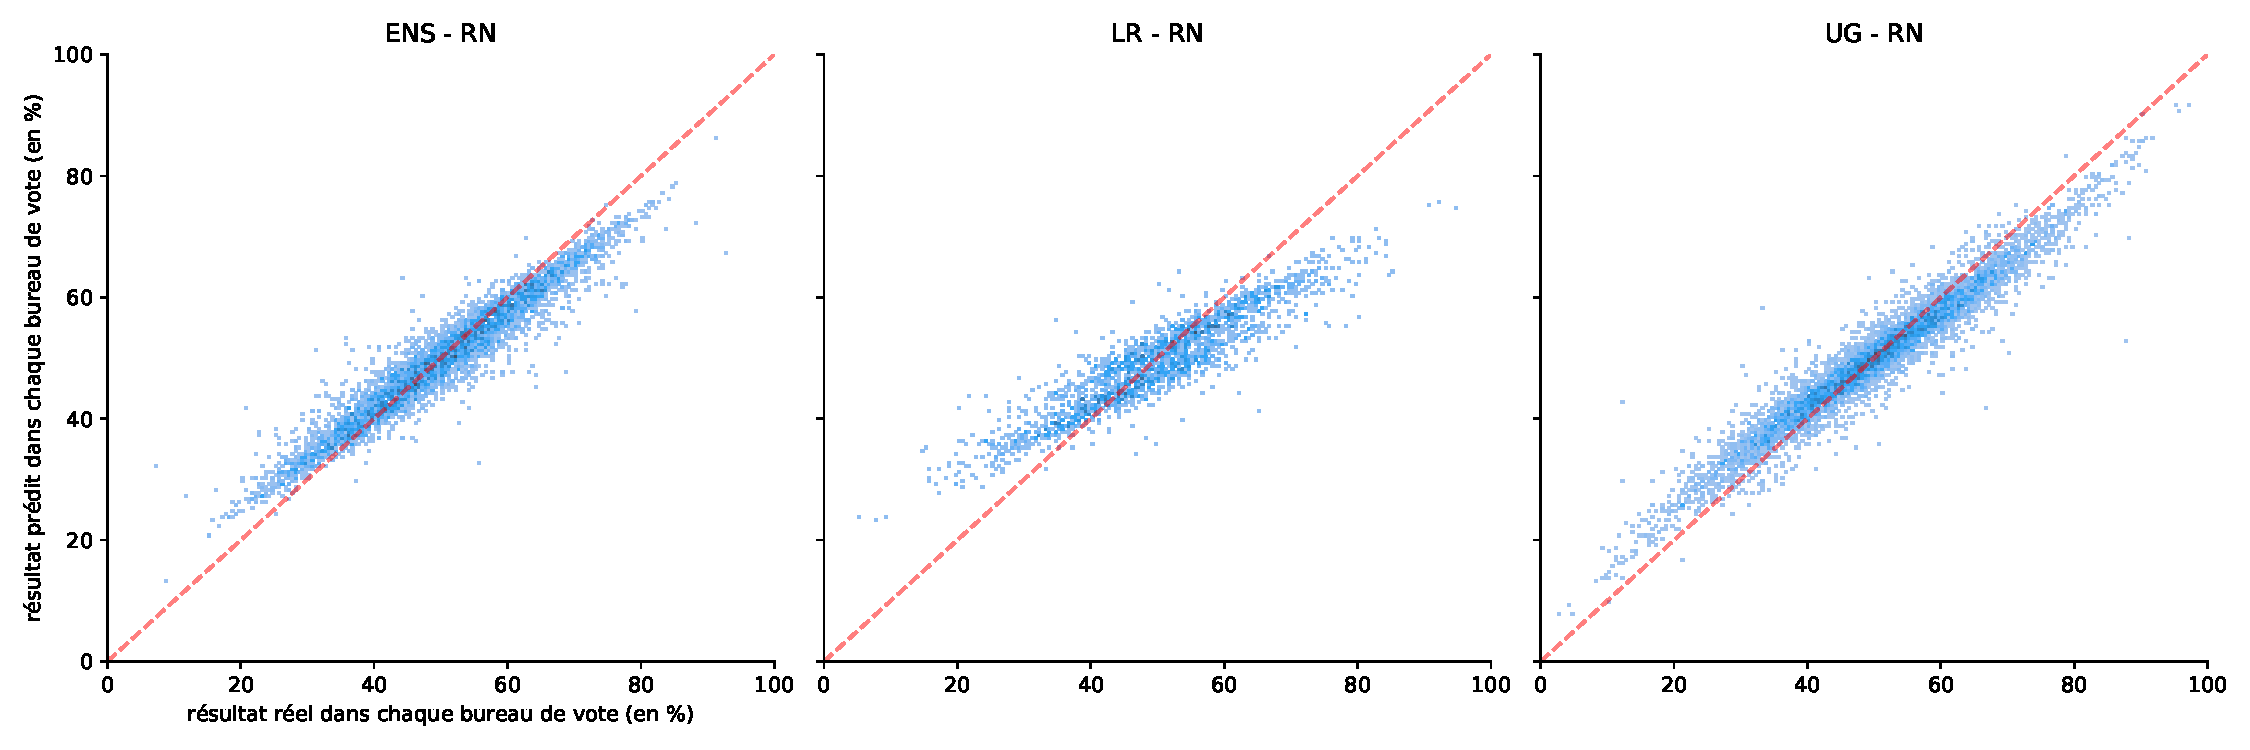
\includegraphics[width=0.9\textwidth]{Focus_True_Pred_Hist.pdf}
                    \caption{Histograme bi-dimensionnel de chaque type de face-à-face du score prédit en fonction du score réel. Créé avec des fenêtres 1\% la couleur indique la densité de point dans la zone.}
                    \label{fig:Focus_pred_true}
                \end{center}
            \end{figure}
            
            \begin{figure}
                \begin{center}
                    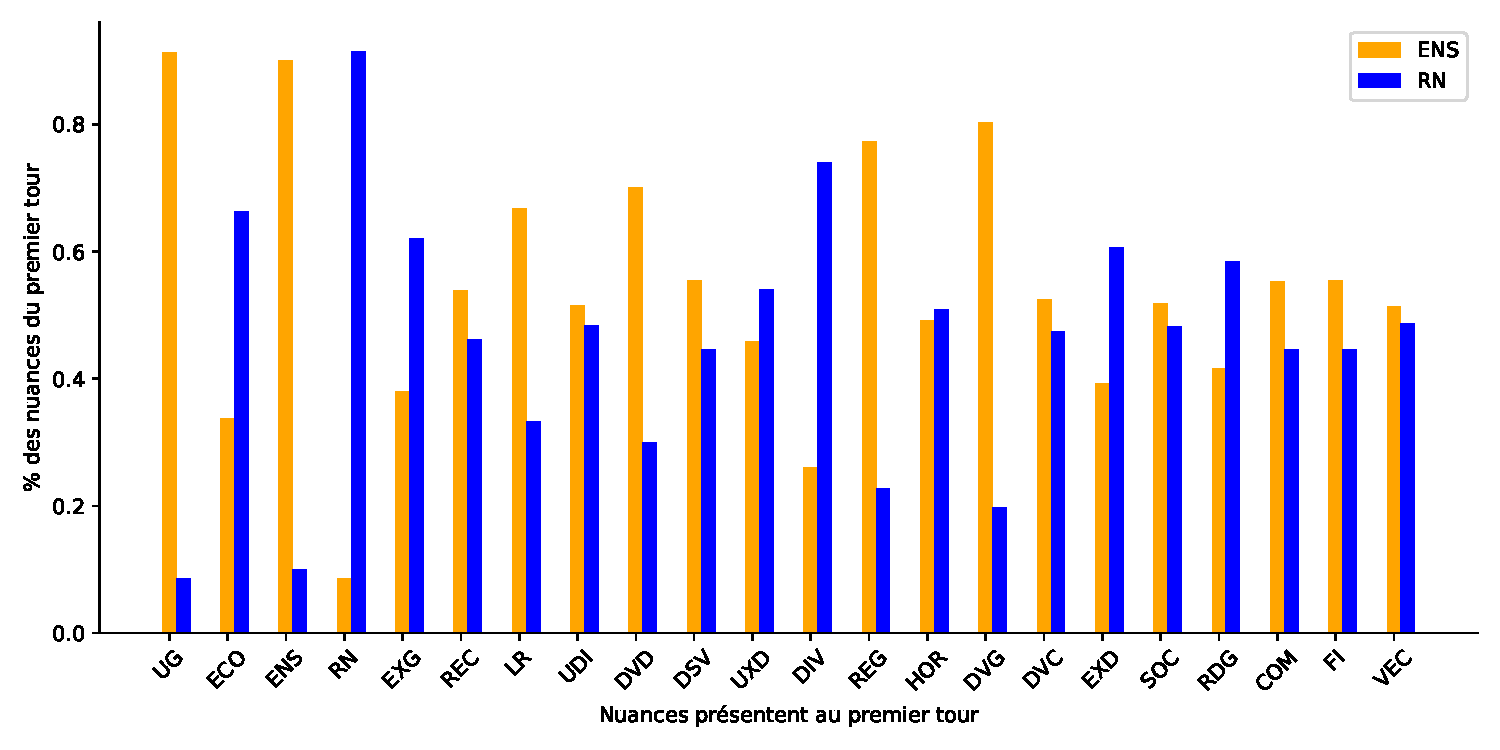
\includegraphics[width=0.7\textwidth]{Focus_ENS_RN.pdf}
                    \caption{Taux de report de chaque parti du premier tour vers l'un des deux candidat du second tour, lors des face-à-face entre ENS et le RN.}
                    \label{fig:ENS-RN}
                \end{center}
            \end{figure}
            \begin{figure}
                \begin{center}
                    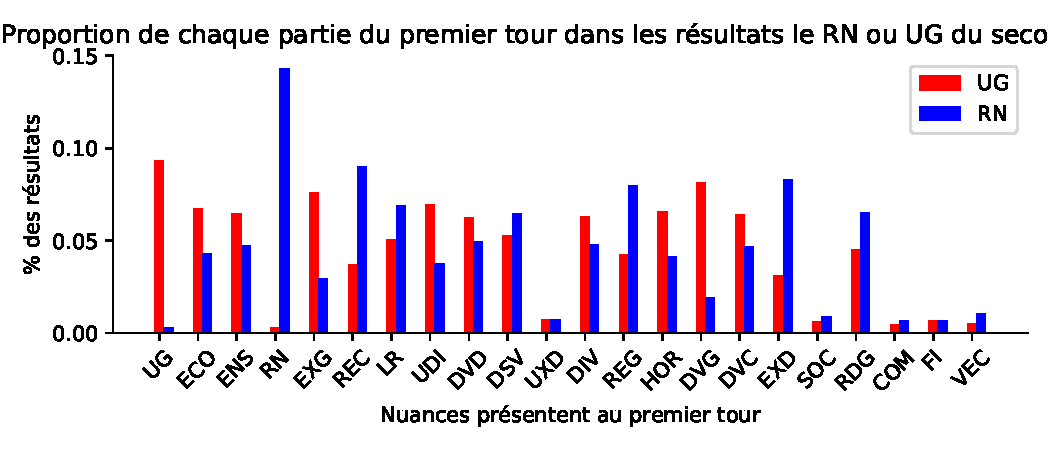
\includegraphics[width=0.7\textwidth]{Focus_UG_RN.pdf}
                    \caption{Taux de report de chaque parti du premier tour vers l'un des deux candidat du second tour, lors des face-à-face entre UG et le RN.}
                    \label{fig:UG-RN}
                \end{center}
            \end{figure}
            \begin{figure}
                \begin{center}
                    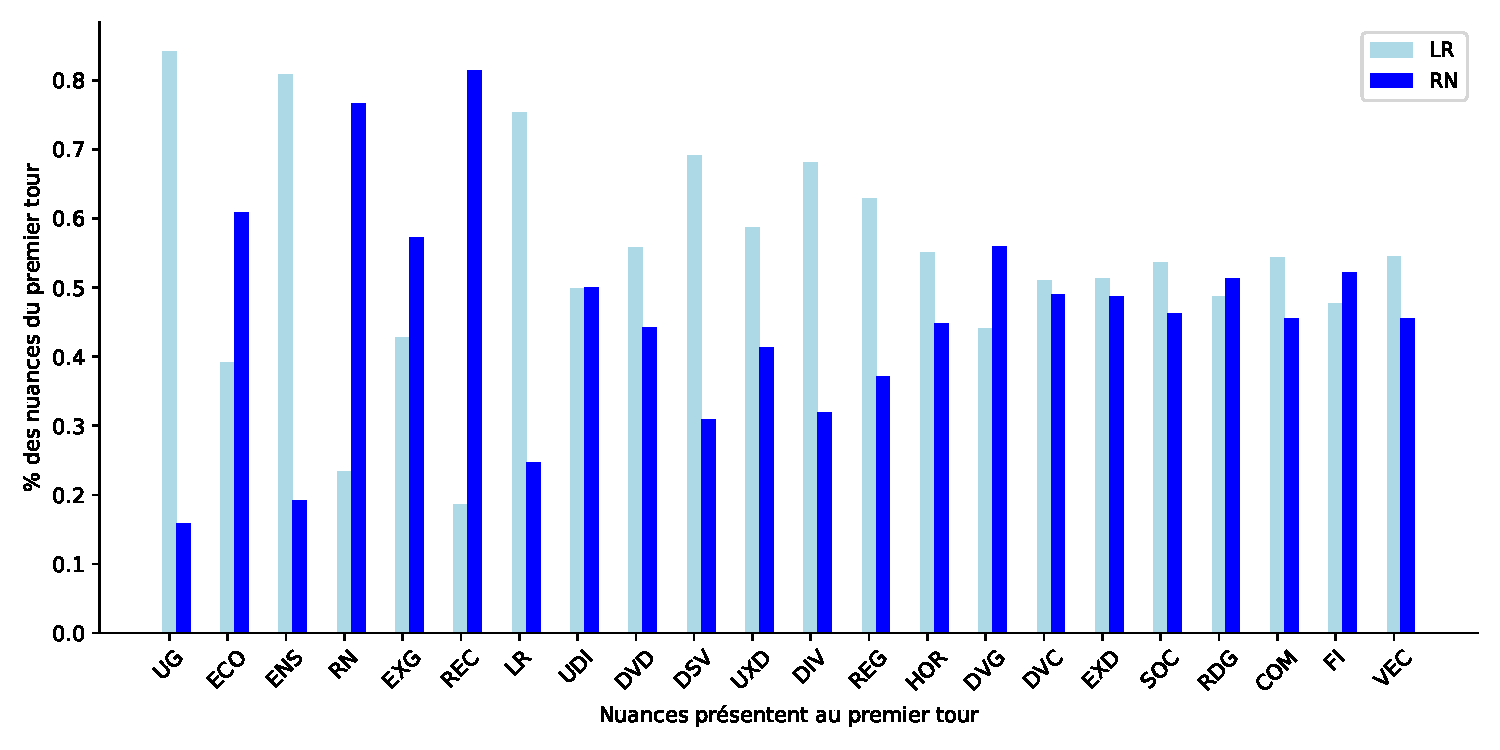
\includegraphics[width=0.7\textwidth]{Focus_LR_RN.pdf}
                    \caption{Taux de report de chaque parti du premier tour vers l'un des deux candidat du second tour, lors des face-à-face entre LR et le RN.}
                    \label{fig:LR-RN}
                \end{center}
            \end{figure}

        \subsection*{Généralisation nationale}
            
            Pour complexifier un peu plus la tâche, et enfin répondre au mieux à notre problématique, il a été possible de considérer le jeu de donné dans son intégralité, et d'en extraire la matrice de transfert permettant de prédire au mieux les résultats du second tour. On remarque alors sur la partie gauche de la figure \ref{fig:True-Pred-Total} une zone large entourant la diagonale rouge. Bien qu'une plus grande densité soit présente autour de cette diagonale, on distingue nettement un second groupe dont les résultats sont sous-évalué par le modèle. Si on se penche alors sur l'extrapolation de la matrice de transfert de voix permettant de représenter les résultats de chaque nuance du second tour, sous la forme d'une somme des partis présent au premier tour, on remarque alors, que la nuance la plus présent pour chaque partis est lui même. Ce taux de A vers A est même majoritaire pour les plus petites nuances (LR, UXD, DVD, HOR, DVC, REG...). Néanmoins, cela est moins juste pour Ensemble et l'Union de la Gauche présentant respectivement 46\% et 32\%, et encore moins pour le Rassemblement National avec seulement 21\%. Se focalisant sur le RN, on remarque que ses voix viendraient principalement de l'Extrême gauche et de Reconquête. Ce dernier est particulièrement présent chez UG et disparaît chez ENS. 

            \begin{figure}[h]
                \begin{center}
                    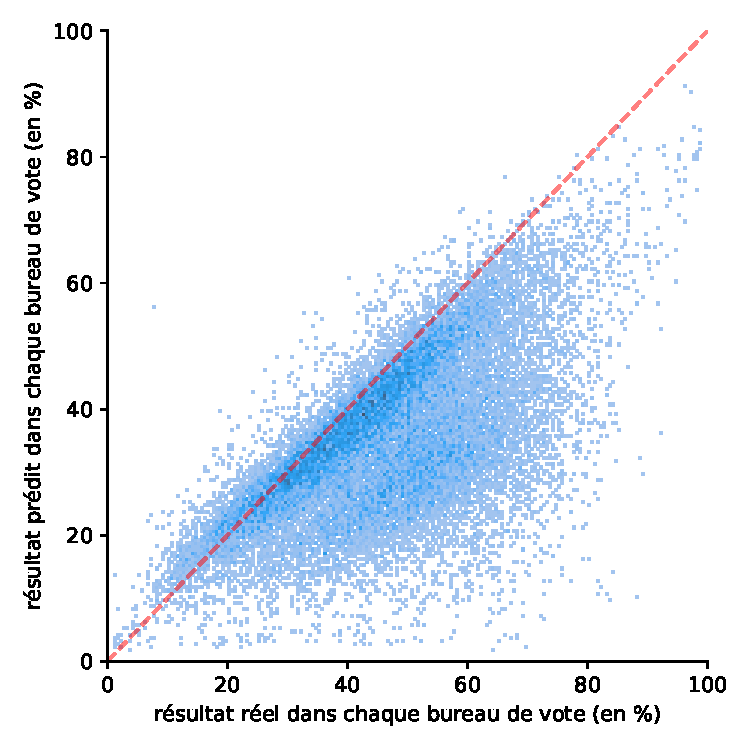
\includegraphics[width=0.3\textwidth]{Total_True_Pred_Hist.pdf}
                    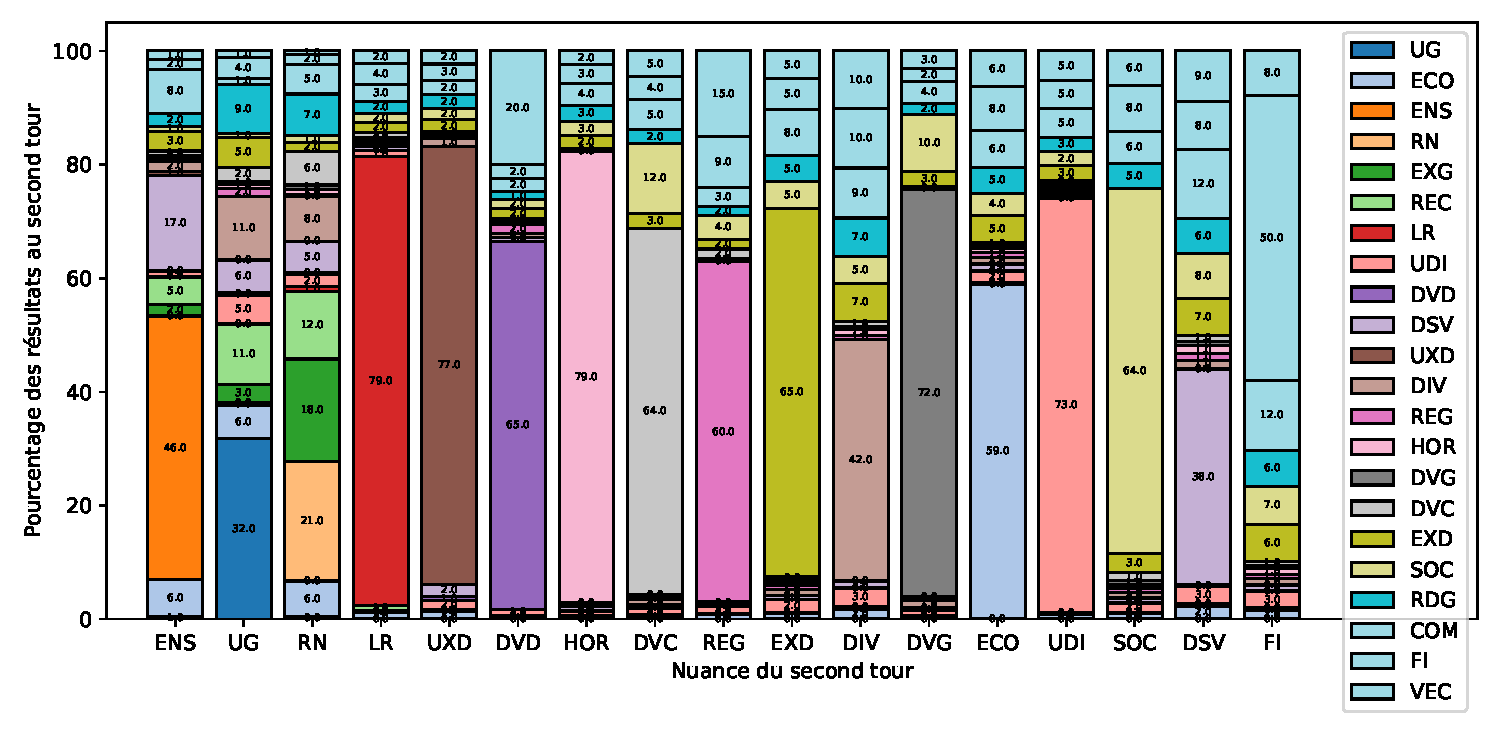
\includegraphics[width=0.65\textwidth]{Total-Matrice-Participation.pdf}
                    \caption{Gauche) Représentation des résultats prédit pour chaque bureau de vote en fonction des résultats réels. Droite) Taux de représentation estimé de chaque nuance du premier tour dans les résultats de chaque nuance du second tour.}
                    \label{fig:True-Pred-Total}
                \end{center}
            \end{figure}
        
    \newpage
    %-------------------------
    % Discussion (1page) + Références
    %-------------------------
    \section{Discussion}
        Ce projet a eu pour objectif de développer une analyse visant à explorer les résultats des élections législatives anticipées de 2024 en France. Le principal objectif était donc de retrouver une matrice permettant de transformer la distribution des votes au premier tour en celle des votes au second. 

        A un niveau très simplifier, le modèle fonctionne mais tend à surestimer ou sous-estimer les résultats, ce qui est probablement dûe une mauvaise répartition des nuances au sein des familles, ainsi que les différence du nombre de votes obtenue au total pour chacune. 
        Lorsque l'on complexifie un peu la tâche en considérant toutes les nuances mais en se concentrant que sur des cas particulier, on remarque que les prédiction sont bien meilleures avec des mouvements plus logiques entre les familles politiques. 

        Enfin, dans le cas le plus complexe, la précision semble bonne, mais on remarque une forte propension du modèle à sous estimer une bonne partie des résultats. Alors qu'un schéma récurrent est qu'une nuance arrivée en tête au premier tour remporte le second tour. Il est important de noter que dans les cas où le Rassemblement National est arrivé en première position au premier tour, certain parti arrivé troisème, et pouvant participer au tour suivant, se sont alors désisté afin de permettre au deuxième de dépasser le RN lors du second tour. Ce "front républicain" va par conséquent à l'encontre du schéma récurrent présenté plus haut et pourrait expliquer une sous-estimation du modèle qui ne prend pas cet élément en considération. 

        Cette méthode permet donc d'estimer une matrice de transition pouvant être assimilé à un report des voix, mais semble quelque peu limiter dans ce contexte par le nombre possible de face-à-face.

    \printbibliography

\end{document}